\chapter{Implementation}
  In this chapter, we will introduce some specifications of the implementation
  of our solution.\\


  \section{General autocorrelation function}
    The autocorrelation function introduced in Equation \eqref{eq:4} can be
    implemented in several ways:

      \subsection{Naive approach}
        The naive approach for the autocorrelation function consists in
        computing all the displacements of the sequence and then
        their correlation with the base sequence as shown in Figure
        \ref{naive_auto:fig:1}. Even though this algorythm it's simple and
        follows the mathematical definition, is too slow. We have to compute
        the correlation function for each component, leading us to a
        complexity of $O(n^{2})$ where n it the size of the sequence with a
        huge constant as we have to build the shifted sequence for each
        component.\\

        This constant can be improved if we avoid building the shifts (just
        using slices of the array), but the complexity would stay the same.

      \subsection{Circular convolution theorem}
        The other option is to step in the world of mathematical properties.
        Fortunatly, there exists the convolution theorem\cite{golomb_ref} that
        lets us express the autocorrelation function in terms of Fourier
        Transforms as:
        \begin{theorem}
          Given a sequence $S$ and the Discrete Fourier Transform($DFT$):
          \begin{equation}
            A(S) = DFT^{-1}[DFT\{S\} · DFT\{S\}^{*}]
          \end{equation}
          where $DFT\{S\}^{*}$ represents the complex conjugate of $DFT\{S\}$.
        \end{theorem}

        Notice that, using the Fast Fourier
        Transform\cite{fast_fourier_transform}, the complexity of this
        method lowers to $O(N log N)$. However, its constant is
        still high as we need to apply 2 FFT to the sequence and apply the
        complex conjugate. In fact, we need to keep in mind that Fourier
        Transforms works with complex components while the naive approach keeps
        using the same type of components which makes its constant even higher
        than the naive approach.

          \begin{figure}
            \inputpython{Chapters/Implementation/naive.py}{0}{100}
            \caption{An example implementation of the naive autocorrelation}
            \label{naive_auto:fig:1}
          \end{figure}

      \subsection{Specific solution for the composition method}

      If we were to use a general method for this computation, we would
      probably use the one based on Fourier Transforms because we will be
      dealing with long sequences that will compensate the big constant of
      this method.\\

      However, we are dealing with sequences with the special property of
      having been built through the composition method. This means that we
      might find a non general way of computing this autocorrelation with better
      computational characteristics.\\

      If we take advantage of Property \ref{composition:prop:1}, we can design
      an algorythm with interesting properties. First of all, the complexity
      function depends on the size of the shift sequence. Being $m$ the
      length of the shift sequence and $n$ the length of the composite
      sequence, the resulting algortyhm has a complexity of $O(nm)$. This means
      that when $m < log(n)$ this algorythm has a better complexity than the
      Fourier Transform's approach.\\

      In addition, this algorythm has a better constant. We just need to
      iterate once through the autocorrelation sequence. This method is more
      cache friendly too as the data source of the function is smaller and it
      doesn't need to use complex operations in binary sequences.\\

      But the biggest improvement in respect of the Fourier Transform is that
      the complexity of a partial result of size $p$ is $O(mp)$ while the
      convolution theorem requires $O(nlog(n))$ for a partial result. In
      practice this means that if we just want to check a certain property
      of the autocorrelation we have no need to compute the whole function.\\

      An example implementation of this algorythm is shown in Figure \ref{composite_auto:fig:1}.

      \begin{figure}[ht!]
        \inputpython{Chapters/Implementation/composite.py}{0}{100}
        \caption{The Cython implementation of the composite autocorrelation.
        Notice that we used branchless programming to improve performance.}
        \label{composite_auto:fig:1}
      \end{figure}

  \section{Single-threaded Branch and Bound}

  The theoretical approach for the Branch and Bound algorithm has already
  explained. In this section, we introduce the actual implementation we used
  in the project in Figure \ref{composite_auto:fig:1}.

  \begin{figure}[ht!]
    \inputpython{Chapters/Implementation/branch_and_bound.py}{0}{100}
    \caption{A Cython implementation of the branch and bound algorythm. Notice
    the amount of extra code to achive C performance.}
    \label{composite_auto:fig:1}
  \end{figure}


  \section{Parallelism model}

  For the parallelism of the project, we decided to work with MPI. This model
  was implemented in pure Python as there was no need for a high performance in
  this part of the software (as the time spent in this code is already
  minimal).\\

  However, we need a low latency assignation of tasks. If we did use shared
  memory, every node would need to access memory through the "slow"
  interconnection network. Instead, with MPI, we can make the proccesses to
  talk between them.\\

  For the purpose of this project, we are going to work with
  MPICH\cite{mpich} as the bindings of MPI4PY support it and it's
  the implementation of the cluster we are working with\cite{calderon}.\\

  In our particular problem, we decided to define a set of tasks to
  distribute between the different nodes. This tasks are subtrees from the
  search space with a given height that defines the size of the task. An
  example is show in Figure \ref{tasks:fig:1}. Notice that the tasks are
  completly unbalanced so a static scheduler wouldn't be efficient at all.\\


  \begin{figure}[ht!]
    \begin{center}
      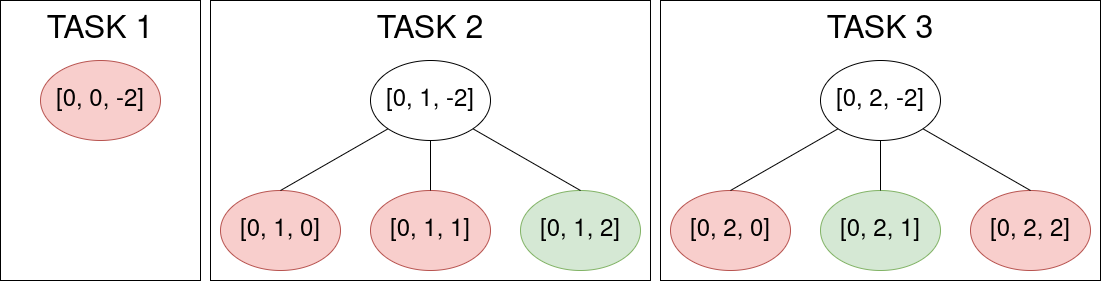
\includegraphics[scale=0.4]{Chapters/Implementation/Example_tasks.png}
    \end{center}
    \caption{An example distribution of tasks for the example at Figure
    \ref{bb:fig:1}.}
    \label{tasks:fig:1}
  \end{figure}

  This model is a good first version. However if we don't prune when assigning
  the tasks we will still have an exponential number of tasks (specifically,
  $n^{l-t}$ where $n$ is the length of the base sequence, $l$ the length of
  the shift sequence and $t$ the task size). This shouldn't be a problem if
  $t$ is close to $l$, but this will raise an issue with the task balancer as
  there wouldn't be enough tasks to balance the load.\\

  A second version of the algorithm applies the branch and bound algorythm in
  the master proccess to generate only tasks with good Hamming properties.
  This rules out all tasks that would instantly result in a bad
  autocorrelation and wouldn't generate any useful sequences. The code
  implementation is shown in Figures \ref{parallelism_example:fig:1} and
  \ref{parallelism_example:fig:2}.\\

  \begin{figure}[ht!]
    \inputpython{Chapters/Implementation/Example_parallelism_master.py}{0}{100}
    \caption{A Python implementation of the master proccess}
    \label{parallelism_example:fig:1}
  \end{figure}

  \begin{figure}[ht!]
    \inputpython{Chapters/Implementation/Example_parallelism_slave.py}{0}{100}
    \caption{A Python implementation of an slave proccess}
    \label{parallelism_example:fig:2}
  \end{figure}

  A third version (which we didn't implement because the second version was
  enough for our objective) could be done by using the Hamming as an
  heuristic to determine the size of the task. Instead of using a fixed size
  for the subtrees, we can give the tasks to the process at hand based on the
  Hamming autocorrelation of the root of the task.\\

  \section{UI implementation}

  Last but not least, we will briefly discuss the design of the User Interface.
  As expressed in the chapter of Sofware Engineering, our primary focus is
  its compatibility with command lines. For that, we used a POSIX compatible
  interface.\\

  First, we provided a --help option to list all the flags:
  \begin{lstlisting}
    $ python main.py --help
    usage: python main.py [option...]

    Options and arguments:
    -n : number of threads to use(must be compatible with your MPI enviroment)
         Defaults to the MPI configuration default

    -p : delay between polls in the master thread(higher values will make the
         slaves to wait more until the next task, lower values will increase
         CPU usage of master)

    -s : length of the base sequence(in this version must be a prime number to
         generate Legendre sequences. Other values have undefined behaviour)

    -l : length of shift sequences(this option must be coprime with value
         of s, other values have undefined behaviour)

    -t : size of the task for each thread(this option must be lower than the
         value provided by -l, other values have undefined behaviour)

    -h : maximum hamming autocorrelation allowed(this option must be a
         positive integer other values have undefined behaviour) Defaults to -l

    -c : maximum autocorrelation we are interested in(this option must be a
         positive integer other values have undefined behaviour) Defaults to
         the square root of (-l*-s)

    -v : verbose mode
  \end{lstlisting}

  Verbose mode logs which tasks have been assigned and at which time stamp, as
  well as logging the end of slave proccesses and the idle time of slaves:

  \begin{lstlisting}
    $ python main.py -s 5 -l 23 -t 20 -c 7 -h 3 -v
    2020-08-23 19:27:49 [1] : TASK_ASSIGNED [0, 0, 1] 9ms
    2020-08-23 19:27:49 [3] : TASK_ASSIGNED [0, 0, 3] 10ms
    2020-08-23 19:27:49 [5] : TASK_ASSIGNED [0, 0, 5] 6ms
    2020-08-23 19:27:49 [7] : TASK_ASSIGNED [0, 1, 1] 17ms
    2020-08-23 19:27:49 [6] : TASK_ASSIGNED [0, 1, 0] 3ms
    2020-08-23 19:27:49 [2] : TASK_ASSIGNED [0, 0, 2] 0ms
                            .
                            .
                            .
    2020-08-23 19:28:41 [1] : TASK_ASSIGNED [0, 5, 0] 0ms
    2020-08-23 19:28:42 [7] : TASK_ASSIGNED [0, 5, 3] 0ms
    2020-08-23 19:28:45 [1] : EXITED
    2020-08-23 19:28:45 [5] : TASK_ASSIGNED [0, 5, 2] 0ms
    2020-08-23 19:28:47 [2] : EXITED
    2020-08-23 19:28:48 [4] : TASK_ASSIGNED [0, 5, 4] 0ms
    2020-08-23 19:28:49 [6] : EXITED
    2020-08-23 19:28:52 [3] : EXITED
    2020-08-23 19:28:55 [5] : EXITED
    2020-08-23 19:28:56 [7] : EXITED
    2020-08-23 19:28:57 [4] : EXITED

  \end{lstlisting}

  Notice that, as we are using stdout, we can pipe the log to a file. The
  output format is designed in a way that eases the use of utilities such as
  awk to proccess the data of the program (one word message, well defined
  columns, etc.).\\

  Verbosity is completly optional and doesn't impact performance when inactive.
  It's particularly useful when tweaking the parameters to get the best
  configuration.\\
